\section{Grundlagen}
\subsection{Schnittstelle}
text

\subsection{REST und RabbitMQ}
\subsubsection{Application Programming Interface}
Ein \ac{api} ist eine Programmierschnittstelle, die dazu da ist, die Kommunikation zwischen einem Client, oder auch Anwender genannt, und einem Server durch festgelegte Funktionen zu regeln. Der Satz der verfügbaren Funktionen ist durch den Entwickler der API vorgegeben. Eine API sollte nach Möglichkeit selbsterklärend aufgebaut sein. \footcite{bloch2006design} Eine API dient dazu, dem Nutzer Daten bereitzustellen oder dem Server Daten zu senden.

In Abbildung 1 ist die Kommunikation zwischen einem Anwender und der API durch ein Sequenzdiagramm dargestellt. Jede Anfrage an die API findet durch den Aufruf des API Endpunkts durch einen \ac{url} statt. Hinter der Grund-URL wird die genaue Ressource innerhalb der API durch den Pfad in der URL angegeben. Jede dieser Funktionen, die über eine bestimmte URL erreichbar sind, kann mehrere Effekte haben. Der Effekt, den die Funktion hat, ist durch die \ac{http} Methoden im groben Rahmen vorgegeben. Die Kommunikation zwischen API und Anwender geht immer vom Anwender aus. Die API kann von sich aus den Anwender nicht ansprechen. 

\begin{figure}[H]
  \centering
    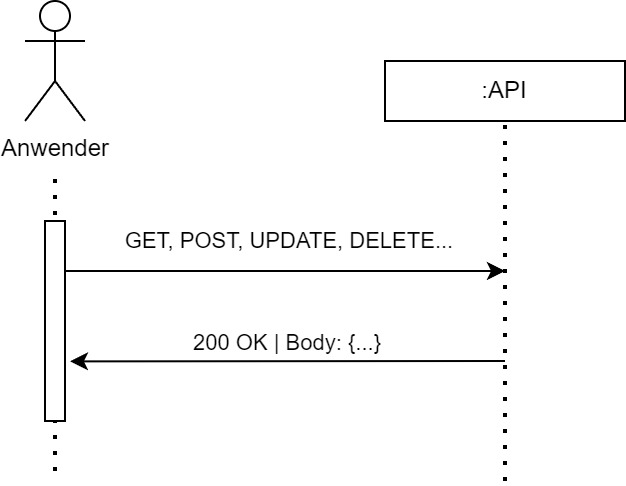
\includegraphics[width = 8cm]{bilder/APISequenzdiagramm}
    \caption{UML Sequenzdiagramm einer API}
\end{figure}

Der gesamte Satz der verfügbaren HTTP-Funktionen lautet \texttt{GET, HEAD, POST, PUT, DELETE, CONNECT, OPTIONS, TRACE, PATCH}. Jede der Funktionen hat eine bestimmte Aufgabe und bestimmte Rechte, die es vom Entwickler der API einzuhalten gilt.\footcite{mdn2022http} In der Bachelorarbeit werden die Funktionen \texttt{GET, POST} und \texttt{DELETE} verwendet. Routen der API, die mit einer \texttt{GET} Funktion aufgerufen werden, sollen lediglich Daten an den Nutzer zurückgeben, ohne Änderungen am Server vorzunehmen. Wenn zwei mal hintereinander die gleiche URL mit \texttt{GET} aufgerufen wird, sollte auch beide male das gleiche Ergebnis von der API zurückgegeben werden.

Die \texttt{POST} Methode liefert Daten vom Nutzer an den Server. Innerhalb des \texttt{POST} Bodys können Daten unter Anderem im JSON Format an die API gesendet werden. API URLs die mit einer \texttt{POST} Methode aufgerufen werden, können Veränderungen auf dem Server auslösen. Dies kann Auswirkungen auf die Daten oder den Status des Servers haben, sodass eventuell andere Methoden davon beeinflusst sind. Ein beispielhafter Anwendungsfall für eine \texttt{POST} Methode ist die Registrierung eines neuen Accounts auf einer Website. Dort wird dann innerhalb des Bodys der Benutzername und das Passwort an die API geschickt. Die API Registriert den Account mit den erhaltenen Daten und gibt bei zukünftigen Aufrufen der URL mit den gleichen Daten einen Fehler zurück, dass der Benutzer bereits registriert ist.

Die \texttt{DELETE} Methode entfernt eine Ressource unter der aufgerufenen URL. Sowohl bei \texttt{POST}, als auch bei \texttt{DELETE} Methoden, ist darauf zu achten, dass der Nutzer die Route nur aufrufen kann, wenn er entsprechende Rechte zur Ausführung verfügt. Ansonsten könnte es zu unkontrollierten Daten- und Statusänderungen innerhalb der API kommen. 

Wie in Abbildung 1 zu sehen ist, gibt die API nicht nur die angeforderten Daten zurück, sondern auch einen Statuscode. Ein HTTP Statuscode besteht aus drei Ziffern. In Tabelle 1 sind die grundlegenden Statuscodes aufgelistet.

\begin{table}[H]
\centering
\begin{tabular}{l|l}
\textbf{Statuscode} & \textbf{Bedeutung} \\
\hline
1xx & Informationen, nur unter HTTP 1.1 definiert \\
2xx & Request war erfolgreich (OK) \\
3xx & Die Ressource wurde verschoben \\
4xx & Die Eingabe war fehlerhaft \\
5xx & Der Server hatte einen Fehler \\
\end{tabular}
\caption{HTTP Statuscodes nach \cite{doglio2015pro}}
\end{table}

Die Statuscodes, die im Prototypen der Bachelorarbeit verwendet wurden, sind Teil der häufiger genutzten Statuscodes für APIs. Der Statuscode \texttt{200:OK} ist der am häufigsten auftretende Statuscode. Dieser besagt, dass die Anfrage erfolgreich abgelaufen ist und das Ergebnis zurückgegeben werden konnte. Der Prototyp nutzt ein Authentifizierungssystem. Dadurch kann es dazu kommen, dass bei einer Anfrage mit fehlender Autorisierung der Statuscode \texttt{401:Unauthorized} zurückgegeben wird. Weitere Statuscodes, die häufiger auftreten können, sind \texttt{404:Not found}, \texttt{405:Method not allowed} und \texttt{500:Internal server error}. Bei einem Statuscode 404 wurde eine Route aufgerufen, die innerhalb der API nicht definiert ist. Bei dem Statuscode 405 wurde zwar eine vorhandene Route angesprochen, jedoch ist die genutzte HTTP Methode nicht zulässig. Der letzte verwendete Statuscode 500 beschreibt einen Serverabsturz bei der Ausführung der Anfrage. 

Die HTTP Methoden und Statuscodes dienen dazu, die Entwicklung und Arbeit mit einer API für den Entwickler einfach zu gestalten. Wie die URLs der API aufgebaut sind und welche HTTP Methoden wann verwendet werden, liegt jedoch vollständig beim Entwickler der API. Um APIs im Allgemeinen etwas zu vereinheitlichen und die Effekte der Funktionen innerhalb der API selbsterklärender werden zu lassen, wurde im Jahr 2000 von Roy Thomas Fielding ein Regelwerk namens \ac{rest} veröffentlicht.\footcite{masse2011rest}

\subsubsection{Representational State Transfer}
Der Representational State Transfer, kurz REST, ist kein spezifischer Standard in der Softwareentwicklung. REST ist eine Richtlinie, die den Aufbau der Kommunikation zu einer API vorgibt. APIs, die das REST-Paradigma implementieren, werden als REST-APIs oder RESTful APIs bezeichnet. Diese bieten damit einen größtenteils standardisierten Weg, Daten zwischen Client und Server auszutauschen. \footcite{richards2006representational}

Innerhalb des REST-Frameworks sind mehrere Aspekte vorgegeben, die eine REST-API ausmachen. Drei der Aspekte sind \glqq Simplizität\grqq{}, \glqq Skalierbarkeit\grqq{} und \glqq Performance\grqq{}. Die Simplizität beschreibt einen allgemeinen, standardisierten Weg, wie der Aufbau und die Kommunikation mit der API ablaufen soll. Dies beinhaltet den Aufbau der Routen und damit der URL, wann Daten an die API geschickt werden sollen, sowie die Form der Daten, die zu versenden sind. 

Die Skalierbarkeit beschreibt das Konzept der beliebigen Erweiterung einer API. Das beinhaltet die Entwicklung der API als solche. Routen und damit Möglichkeiten, Daten von der API anzufordern oder Daten an die API zu senden, können während der Entwicklung einfach hinzugefügt und entfernt werden. Das Konzept der Skalierbarkeit beschreibt ebenfalls einen zustandslosen Aufbau der API. Durch die Zustandslosigkeit, kann die API horizontal skaliert werden. Eine horizontale Skalierung beschreibt das hinzufügen neuer Instanzen der API. Jede Instanz ist identisch aufgebaut und kann jede ankommende Anfrage alleinstehend beantworten. Die Anfragen, die an eine REST-API gestellt werden, müssen daher alle, für die Bearbeitung notwendigen, Informationen bereitstellen.

Der letzte Aspekt des REST-Frameworks beschreibt die Performance. Eine REST-API implementiert ein System zum Zwischenspeichern, auch Cachen gennant, von Responses. Wenn ein Client eine Anfrage mit der HTTP Methode GET an die API schickt, wird die Antwort, die an den Client zurückgesendet wird auf dem Server zwischengespeichert. Sollte ein oder mehrere Clients eine identische Anfrage an die API senden, wird das zwischengespeicherte Ergebnis zurückgegeben, statt die dahinter liegende Methode innerhalb der API neu auszuführen. Das ermöglicht eine hohe Performance, auch bei einer großen Anzahl von Anfragen.\footcite{fielding2000rest}


\subsubsection{RabbitMQ}
%Genauer auf die Funktionsweise RabbitMQ eingehen
Kommunikation ist für den Aufbau von komplexen Strukturen essenziell. Das betrifft zum Beispiel die natürliche Sprache der Menschen, damit das Leben in einer Gesellschaft möglich wird. Für komplexe Programme in der \ac{it} gelten die gleichen Prinzipien. \footcite{dossot2014rabbitmq}

Bei einer grundlegenden Kommunikation gibt es zwei Kommunikationspartner, einen Sender und einen Empfänger. Im Bereich der Software ist der Sender meist ein Client und der Empfänger ein Server, der öffentlich erreichbar ist. Der Client sendet eine Anfrage, der auch Request genannt wird, an den Server. Anschließend wartet der Client auf eine Antwort. Der Server erhält den Request und verarbeitet ihn. Es wird abhängig vom Request eine Antwort, die als Response bezeichnet wird, generiert und dem Client zurückgesendet. Der Client erhält die Response und schließt damit den Kommunikationsvorgang ab. Dieser Ablauf ist in Abbildung 1 visualisiert.
\begin{figure}[H]
  \centering
    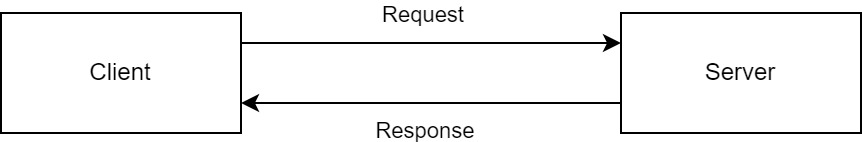
\includegraphics[width = 12cm]{bilder/Rabbit1}
    \caption{Grundlegende Kommunikation}
\end{figure}

Durch die Art der synchronen Kommunikation sind Client und Server sehr eng miteinander Verbunden. Wenn der Client erwartet eine Response von genau dem Server, an den er den Request geschickt hat. Das macht die Skalierung und Ausfallsicherheit allerdings relativ schwierig.

Damit eine Kommunikation zwischen unabhängigen Programmen möglich wird, muss es einen Zwischendienst geben, der die Nachrichten von einem Programm zum anderen transportiert. Bei der Kommunikation zwischen einer Website und einer API wird HTTP verwendet. Dieses stellt sicher, dass die die Nachrichten erfolgreich beim Empfänger ankommen. Sollte eine Nachricht nicht angekommen sein, hat der Absender die Möglichkeit, die Nachricht erneut zu schicken. Über HTTP wird automatisch eine erneute Anfrage geschickt, wenn keine Antwort vom Server zurück kam. Problematisch wird diese Herangehensweise, wenn die Antwortzeit sehr lang wird oder ungewiss ist, ob überhaupt eine Antwort kommen wird. 

RabbitMQ ist ein eine nachrichtenorientierte Middleware, die eine Kommunikation zwischen zwei oder mehreren Programmen durch das \ac{amqp} ermöglicht. RabbitMQ dient als Broker, der Nachrichten von mehreren Clients an mehrere Server vermitteln kann. Im Gegensatz zu einer direkten Kommunikation zwischen Client und Server wie bei HTTP, wird in RabbitMQ eine Queue implementiert, in der alle Anfragen gesammelt werden. 

Eine Queue ist eine Datenstruktur die mehrere Operationen definiert werden. Die Queue fungiert als Warteschlange, in der Einträge gespeichert und in der Reihenfolge des Eingangs auch wieder ausgelesen werden können. Sie funktioniert nach dem First In - First Out, kurz FIFO, Prinzip. Es wird eine \texttt{push} Operation definiert, mit der ein Eintrag an den Anfang der Warteschlange geschrieben wird. Des Weiteren gibt es eine \texttt{pop} Operation, die das älteste Element aus der FIFO Queue ausliest und es aus der Warteschlange entfernt.

Jeder Client kann Nachrichten in die Queue schreiben. Diese Nachrichten werden dort so lange gespeichert, bis sie von einem Dienst ausgelesen werden. In Abbildung 2 ist die Kommunikation zwischen Client und Server mittels eines Brokers abgebildet.
 
\begin{figure}[H]
  \centering
    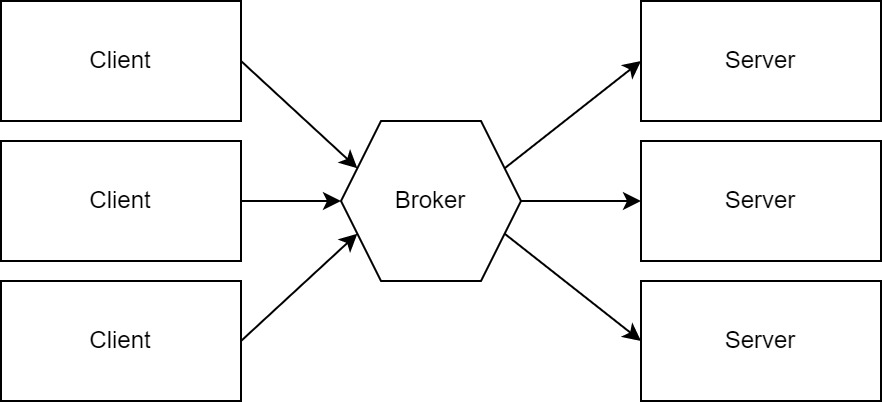
\includegraphics[width = 12cm]{bilder/Rabbit2}
    \caption{Kommunikation über einen Broker}
\end{figure}

Durch diese Herangehensweise wird eine asynchrone Kommunikation zwischen Client und Server ermöglicht. Da RabbitMQ frei von den Handshakes des HTTP ist, sind die Schreib- und Lesezeiten deutlich schneller.\footcite{ionescu2015analysis}

Die Middleware RabbitMQ wird für die Kommunikation zwischen der Flask API und den KI-Services genutzt. Der im Frontend vom Nutzer eingegebene Text-Input wird an die Flask API geschickt. Die Flask API modifiziert den Text im Anschluss so, dass es mittels der \ac{json} über den RabbitMQ Service in die Queue geschrieben werden kann. Jeder KI-Service hat eine Queue einprogrammiert, aus der die Nachrichten ausgelesen werden. Diese Nachrichten können dann verarbeitet und im Anschluss in eine Response-Queue geschrieben werden. Das Flask Backend kann diese Response-Queue auslesen und die einzelnen Antworten zusammenbauen.

\subsection{Künstliche Intelligenz}
text\footcite{gorz2010handbuch}
\subsubsection{Grundlagen einer KI}
%recherche!

\subsubsection{Künstliche Intelligenz als Service}
%aus projektergebnissen
%oftmals Blackbox von Drittanbieter
Die KI-Services sind alleinstehende Programme, die die Aufgabe haben, Nachrichten anzunehmen, sie zu transformieren, zu analysieren und anschließend ein oder mehrere Ergebnisse zurückzugeben. 

Um die Nachrichten empfangen und die Ergebnisse zurücksenden zu können, muss in jedem Service eine AMQP Verbindung zu RabbitMQ hergestellt werden.

Im Prototypen zur Anbindung von austauschbaren Datenquellen an KI-Algorithmen wurde ein Service zur Textähnlichkeitssuche implementiert. Dieser nimmt nutzt das \ac{bert} Modell von Google. Beim Starten des Services werden alle Einträge in einer Elasticsearch Datenbank mithilfe der künstlichen Intelligenz analysiert und in semantische Vektoren konvertiert. Der Service kann anschließend vom Nutzer eingegebene Anfragen mit dem gleichen BERT Modell analysieren und den daraus entstandenen Vektor mit den Vektoren in der Datenbank abgleichen. Nach einem erfolgreichen Suchdurchlauf werden die semantisch ähnlichsten Einträge über RabbitMQ wieder an das Backend zurückgegeben.

\subsection{Microservice Architekturen}
text
\subsection{Verwendete Werkzeuge}
\subsubsection{Python API mit Flask}
%Implementierung der Rest api durch Flask
Python ist eine um 1991 von Guido van Rossum entwickelte Programmiersprache. Bei der Entwicklung von Python wurde ein besonderer Fokus auf die Lesbarkeit von Code gesetzt. Dank der simplifizierten Syntax im Vergleich zu anderen höheren Programmiersprachen wie Java oder C\#, ist Python auch in Bereichen, wie in der Mathematik oder der Wissenschaft ein häufig genutztes Werkzeug. Python bietet ebenfalls die Möglichkeit, von anderen Entwicklern bereitgestellte Bibliotheken in das eigene Projekt zu integrieren.\footcite{python2021python} 

Flask ist eine der verfügbaren Bibliotheken, die ein Framework für die Implementierung einer webbasierten API bereitstellt. Eine API dient dazu, Funktionen und Routen zu definieren, um die Kommunikation zwischen dem Frontend und dem Backend herzustellen. Das Flask Framework ist im Gegensatz zu anderen Frameworks sehr klein. Dies ermöglicht ein schnelles aufsetzen und entwickeln. Da Flask nur die nötigsten Grundlagen für eine API mitliefert, ist der Code besser lesbar und damit für andere Entwickler besser wartbar.\footcite{grinberg2018flask} 

Die Flask API wird für die Anbindung des Frontends an die Datenbank, sowie die Anbindung an die Kommunikationsschnittstelle von RabbitMQ verwendet. Sie nimmt die Daten oder die Eingaben des Nutzers entgegen und vermittelt sie an den richtigen Dienst, damit sie von einer KI-Schnittstelle ausgewertet werden können. Anschließend kann die API angefragt werden, ob es bereits Antworten von einer \ac{ki} zu der vorher geschickten Anfrage gab. Falls die API die Auswertung der KI erhalten hat, wird diese für das Frontend bereitgestellt, um sie dort anzeigen zu können.  

\subsubsection{REDIS und MySQL Datenbanken}
Redis ist eine In-Memory Key-Value Datenbank. Im Gegensatz zu  \ac{rdbms} wie MySQL oder PostgreSQL werden in Redis keine festen Tabellenstrukturen hinterlegt. Redis gehört damit zur Kategorie der NoSQL Datenbanken (Not Only SQL). Key-Value Stores sind kein Ersatz für eine relationale Datenbank, bieten aber für bestimmte Bereiche große Vorteile. Durch das Fehlen von komplexen Strukturen innerhalb der Datenbank kann Redis Anfragen weitaus schneller als andere Datenbanksysteme bearbeiten. Da Redis im \ac{ram} ausgeführt wird,  werden die Daten grundsätzlich nicht persistent gespeichert. ACID (Atomicity, Consistency, Durability and Isolation) Konformität wird mit Redis ebenfalls nicht gewährleistet. Für den Einsatzzweck als Cache in einer Cloud Umgebung ist Redis allerdings sehr gut geeignet. \footcite{paksula2010persisting}

Innerhalb des Redis Key-Value Stores werden alle relevanten Daten gespeichert, die ein Nutzer während seiner Benutzung der Software produziert. Dort werden ebenfalls die Zwischenergebnisse abgespeichert, die die KI während der Analyse erstellt.
%
%\subsection{MySQL Datenbank für Services und Logs}
MySQL ist ein um 1995 erschienenes Open-Source RDBMS. MySQL ist eines der weitverbreitetsten und schnellsten Datenbanksysteme in seiner Kategorie. \footcite{dubois2008mysql}

In relationalen Datenbanken werden Daten strukturiert in Tabellenform abgespeichert. Einzelne Tabellen können Verlinkungen und Referenzen auf andere Tabellen haben, damit die Zusammengehörigkeit der Daten beschrieben werden kann, ohne Daten redundant speichern zu müssen. In MySQL, wie auch anderen RDBMS, werden Tabellenstrukturen und Daten persistent abgespeichert. In-Memory Datenbanken wie Redis können Daten über Umwege auch persistent speichern, jedoch müssen dafür größere Anpassung an der Konfiguration von Redis vorgenommen werden.

Das RDBMS MySQL wird unter Anderem für die Speicherung der Logs, die der Flask Server während der Verarbeitung von Requests oder Nachrichten an die KI produziert, verwendet. Ein weiterer Einsatzzweck der MySQL Datenbank ist die Speicherung der im System registrieren KI-Services. Ein Dienst kann über die Flask API im System registriert oder deregistriert werden. Das Frontend kann im Anschluss eine Auflistung der verfügbaren Services beim Backend anfragen.

\subsubsection{Angular Frontend}
Eine grundlegende Website wird klassisch mit \ac{html} und JavaScript erstellt. Um eine moderne Website zu entwickeln, die ihren Inhalt nicht beim ersten Aufrufen lädt, sondern erst dann, wenn er benötigt wird, müssen Konzepte wie \ac{ajax} verwendet werden. Angular ist ein von Google entwickeltes und gepflegtes Open Source Framework, welches das Entwickeln von komplexen webbasierten Anwendungen vereinfachen soll. Angular bietet im Gegensatz zu anderen Webframeworks wie React und Vue.js eine vollumfängliche Bibliothek, mit der nahezu alle Aspekte in der Web Entwicklung abgedeckt werden können.\footcite{moiseev2018angular}

In Angular wird die Programmiersprache TypeScript verwendet. Diese ist eine Erweiterung der Programmiersprache JavaScript und implementiert Konzepte wie feste Typisierung von Variablen. Weitere Konzepte wie Dependency Injection oder die Trennung von \ac{bl} und \ac{ui} ermöglichen eine schnelle Entwicklung von komplexen Systemen. 

Das Frontend wird für die Ein- und Ausgabe der Daten verwendet. Der Nutzer kann auf der Webseite seine Suchanfrage in ein Textfeld schreiben und anschließend auf den Server hochladen. Im nächsten Schritt wird die Möglichkeit bereitgestellt, die eingegeben Daten automatisiert zu bearbeiten und zu manipulieren. Im gleichen Zug wird die Eingabe des Nutzers in ein für die KI verständliches Format konvertiert. Im letzten Schritt kann der Nutzer die Anfrage an das Backend schicken, dass mit der Analyse der Eingabe begonnen werden soll. Das Frontend fängt daraufhin an beim Backend in regelmäßigen Abständen nach Antworten der KI zu fragen. Wenn Antworten vorhanden sind, können diese in einer Liste visualisiert werden.


\subsubsection{Logging durch Grafana}
Grafana ist ein von Torkel Ödegaard in 2014 entwickeltes Open-Source Datenvisualisierungsprogramm. Grafana kann zeitbasierte Daten in verschiedenen Arten von Grafen und Diagrammen anzeigen.\footcite{chakraborty2021grafana}

Eines der möglichen Panels für ein Dashbaord ist das Log-Panel. Dort werden die Log Nachrichten aus einer Datenbank angezeigt und mit einer Farbe, abhängig vom Schweregrad markiert. Als Datenquelle können unter Anderem zeitbasierte Datenbanken wie InfluxDB und Prometheus oder RDBMS wie MySQL verwendet werden.

Im implementierten Prototypen wurde eine MySQL verwendet, in der die zu loggende Nachricht, der Schweregrad, ein Zeitstempel und die User \ac{id} gespeichert werden. Diese Daten werden verwendet, um die Logs im Log-Panel von Grafana chronologisch anzeigen zu lassen.

\subsubsection{Deployment über Docker}
Docker ist eine Software zur Virtualisierung von Containern. Ein Container beschreibt eine in sich geschlossene Umgebung, in der ein Programm ausgeführt werden kann. Alle benötigten Dateien, Parameter und Umgebungsvariablen werden beim Starten des Containers mitgegeben. Damit kann sichergestellt werden, dass ein Programm, welches innerhalb eines Docker Containers ausgeführt wird, sich in jeder Umgebung gleich verhält. Hierdurch wird die Unabhängigkeit vom Host-Betriebsystem gewährleistet. Im Gegensatz zu einer \ac{vm} muss für die Ausführung eines Docker Containers kein komplettes Betriebssystem virtualisiert werden. Das Hochfahren einzelner Container ist deutlich schneller und ressourcenschonender als die Implementierung einzelner VMs.\footcite{anderson2015docker}

Des Weiteren können über das Docker Compose Plugin mehrere Container gleichzeitig hochgefahren werden, sodass mit einer einzigen Kommandozeileneingabe eine komplette Softwarearchitektur hochgefahren werden kann.

Docker wird für das Deployment der einzelnen Komponenten des Prototyps verwendet. Für Redis, MySQL, RabbitMQ, Grafana und Elasticsearch können die benötigten Images, die eine Bauanleitung darstellen, aus dem Docker Hub heruntergeladen und genutzt werden. In einem Docker Image sind auch alle für die Ausführung des Programms benötigten Dateien gepackt. Docker Hub ist eine Plattform zur Verteilung von offiziellen Docker Images, von der automatisch alle Images runtergeladen werden, die lokal nicht vorhanden sind.

Für das Angular Frontend und das Flask Backend müssen die Images erst manuell gebaut werden, bevor sie als Container gestartet werden können. Dafür bietet die Docker sogenannte Dockerfiles an, in der die benötigten Konfigurationen hinterlegt werden können.

